

\tikzset{every picture/.style={line width=0.75pt}} %set default line width to 0.75pt        

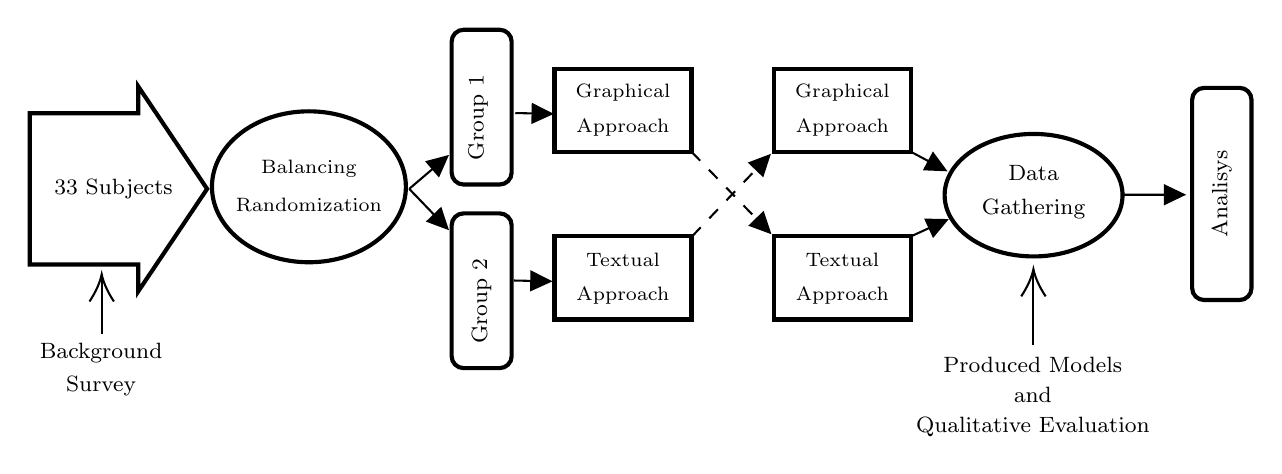
\begin{tikzpicture}[x=0.9pt,y=0.9pt,yscale=-1,xscale=1]
%uncomment if require: \path (0,327); %set diagram left start at 0, and has height of 327


%Shape: Ellipse [id:dp633810982278807] 
\draw  [line width=1.5]  (84.73,72.26) .. controls (84.73,55.52) and (102.16,41.96) .. (123.66,41.96) .. controls (145.16,41.96) and (162.59,55.52) .. (162.59,72.26) .. controls (162.59,88.99) and (145.16,102.56) .. (123.66,102.56) .. controls (102.16,102.56) and (84.73,88.99) .. (84.73,72.26) -- cycle ;



%Shape: Ellipse [id:dp7904221795411808] 
\draw  [line width=1.5]  (378.89,75.63) .. controls (378.89,62.05) and (394.88,51.04) .. (414.61,51.04) .. controls (434.33,51.04) and (450.32,62.05) .. (450.32,75.63) .. controls (450.32,89.21) and (434.33,100.22) .. (414.61,100.22) .. controls (394.88,100.22) and (378.89,89.21) .. (378.89,75.63) -- cycle ;

%Rounded Rect [id:dp5302697683495847] 
\draw  [line width=1.5]  (180.95,87.75) .. controls (180.95,85.09) and (183.11,82.93) .. (185.77,82.93) -- (200.23,82.93) .. controls (202.9,82.93) and (205.06,85.09) .. (205.06,87.75) -- (205.06,140.25) .. controls (205.06,142.91) and (202.9,145.07) .. (200.23,145.07) -- (185.77,145.07) .. controls (183.11,145.07) and (180.95,142.91) .. (180.95,140.25) -- cycle ;
%Rounded Rect [id:dp9616486966995694] 
\draw  [line width=1.5]  (180.95,14.03) .. controls (180.95,11.37) and (183.11,9.21) .. (185.77,9.21) -- (200.23,9.21) .. controls (202.9,9.21) and (205.06,11.37) .. (205.06,14.03) -- (205.06,66.52) .. controls (205.06,69.19) and (202.9,71.35) .. (200.23,71.35) -- (185.77,71.35) .. controls (183.11,71.35) and (180.95,69.19) .. (180.95,66.52) -- cycle ;

%Shape: Rectangle [id:dp03801896284105699] 
\draw  [line width=1.5]  (222.23,24.87) -- (277.28,24.87) -- (277.28,58.21) -- (222.23,58.21) -- cycle ;
%Straight Lines [id:da1799424135415575] 
\draw    (163.93,73.09) -- (177.61,61.43) ;
\draw [shift={(179.89,59.48)}, rotate = 499.54] [fill={rgb, 255:red, 0; green, 0; blue, 0 }  ][line width=0.08]  [draw opacity=0] (8.93,-4.29) -- (0,0) -- (8.93,4.29) -- cycle    ;
%Straight Lines [id:da17029537209985257] 
\draw    (163.93,73.09) -- (177.81,87.53) ;
\draw [shift={(179.89,89.69)}, rotate = 226.13] [fill={rgb, 255:red, 0; green, 0; blue, 0 }  ][line width=0.08]  [draw opacity=0] (8.93,-4.29) -- (0,0) -- (8.93,4.29) -- cycle    ;
%Straight Lines [id:da39402523544663426] 
\draw  [dash pattern={on 4.5pt off 4.5pt}]  (277.5,92.15) -- (307.06,61.21) ;
\draw [shift={(309.13,59.04)}, rotate = 493.69] [fill={rgb, 255:red, 0; green, 0; blue, 0 }  ][line width=0.08]  [draw opacity=0] (8.93,-4.29) -- (0,0) -- (8.93,4.29) -- cycle    ;
%Straight Lines [id:da7992081880522388] 
\draw  [dash pattern={on 4.5pt off 4.5pt}]  (277.28,58.21) -- (307.27,89.16) ;
\draw [shift={(309.35,91.31)}, rotate = 225.9] [fill={rgb, 255:red, 0; green, 0; blue, 0 }  ][line width=0.08]  [draw opacity=0] (8.93,-4.29) -- (0,0) -- (8.93,4.29) -- cycle    ;
%Right Arrow [id:dp3913444800583221] 
\draw  [line width=1.5]  (11.57,42.74) -- (55.14,42.74) -- (55.14,31.99) -- (82.78,73.11) -- (55.14,114.23) -- (55.14,103.49) -- (11.57,103.49) -- cycle ;
%Shape: Rectangle [id:dp003852149638719382] 
\draw  [line width=1.5]  (310.31,24.87) -- (365.36,24.87) -- (365.36,58.21) -- (310.31,58.21) -- cycle ;
%Shape: Rectangle [id:dp0126542660109914] 
\draw  [line width=1.5]  (310.31,92.18) -- (365.36,92.18) -- (365.36,125.52) -- (310.31,125.52) -- cycle ;
%Shape: Rectangle [id:dp4954877903085966] 
\draw  [line width=1.5]  (222.23,92.18) -- (277.28,92.18) -- (277.28,125.52) -- (222.23,125.52) -- cycle ;
%Straight Lines [id:da3442884963113835] 
\draw    (365.36,58.21) -- (377.4,64.63) ;
\draw [shift={(380.04,66.05)}, rotate = 208.07999999999998] [fill={rgb, 255:red, 0; green, 0; blue, 0 }  ][line width=0.08]  [draw opacity=0] (8.93,-4.29) -- (0,0) -- (8.93,4.29) -- cycle    ;
%Straight Lines [id:da6883068419855551] 
\draw    (365.36,92.18) -- (377.84,86.46) ;
\draw [shift={(380.57,85.22)}, rotate = 515.4100000000001] [fill={rgb, 255:red, 0; green, 0; blue, 0 }  ][line width=0.08]  [draw opacity=0] (8.93,-4.29) -- (0,0) -- (8.93,4.29) -- cycle    ;
%Rounded Rect [id:dp5928061300931144] 
\draw  [line width=1.5]  (478.27,37.32) .. controls (478.27,34.68) and (480.41,32.55) .. (483.04,32.55) -- (497.34,32.55) .. controls (499.97,32.55) and (502.1,34.68) .. (502.1,37.32) -- (502.1,112.96) .. controls (502.1,115.59) and (499.97,117.72) .. (497.34,117.72) -- (483.04,117.72) .. controls (480.41,117.72) and (478.27,115.59) .. (478.27,112.96) -- cycle ;

%Straight Lines [id:da6932528701926595] 
\draw    (450.32,75.46) -- (472.85,75.45) ;
\draw [shift={(475.85,75.45)}, rotate = 539.96] [fill={rgb, 255:red, 0; green, 0; blue, 0 }  ][line width=0.08]  [draw opacity=0] (8.93,-4.29) -- (0,0) -- (8.93,4.29) -- cycle    ;
%Straight Lines [id:da7950818392289087] 
\draw    (40.46,131.56) -- (40.46,109.39) ;
\draw [shift={(40.46,107.39)}, rotate = 450] [color={rgb, 255:red, 0; green, 0; blue, 0 }  ][line width=0.75]    (10.93,-4.9) .. controls (6.95,-2.3) and (3.31,-0.67) .. (0,0) .. controls (3.31,0.67) and (6.95,2.3) .. (10.93,4.9)   ;
%Straight Lines [id:da5784112946450906] 
\draw    (414.54,135.73) -- (414.54,107.33) ;
\draw [shift={(414.54,105.33)}, rotate = 450] [color={rgb, 255:red, 0; green, 0; blue, 0 }  ][line width=0.75]    (10.93,-4.9) .. controls (6.95,-2.3) and (3.31,-0.67) .. (0,0) .. controls (3.31,0.67) and (6.95,2.3) .. (10.93,4.9)   ;
%Straight Lines [id:da04489153588175898] 
\draw    (206.5,42.65) -- (218.97,42.92) ;
\draw [shift={(221.97,42.99)}, rotate = 181.23] [fill={rgb, 255:red, 0; green, 0; blue, 0 }  ][line width=0.08]  [draw opacity=0] (8.93,-4.29) -- (0,0) -- (8.93,4.29) -- cycle    ;
%Straight Lines [id:da30869554668079413] 
\draw    (205.97,109.89) -- (218.45,110.16) ;
\draw [shift={(221.44,110.22)}, rotate = 181.23] [fill={rgb, 255:red, 0; green, 0; blue, 0 }  ][line width=0.08]  [draw opacity=0] (8.93,-4.29) -- (0,0) -- (8.93,4.29) -- cycle    ;




% Text Node
\draw (249.75,48.63) node  [font=\scriptsize] [align=left] {Approach};
% Text Node
\draw (249.75,34.46) node  [font=\scriptsize] [align=left] {Graphical};
% Text Node
\draw (490.19,75.14) node  [font=\footnotesize,rotate=-270] [align=left] {Analisys};
% Text Node
\draw (414.31,168.64) node  [font=\footnotesize] [align=left] {Qualitative Evaluation};
% Text Node
\draw (414.31,155.81) node  [font=\footnotesize] [align=left] {and};
% Text Node
\draw (414.31,143.84) node  [font=\footnotesize] [align=left] {Produced Models};
% Text Node
\draw (187.85,136.5) node [anchor=north west][inner sep=0.75pt]  [font=\footnotesize,rotate=-270] [align=left] {Group 2};
% Text Node
\draw (337.84,34.46) node  [font=\scriptsize] [align=left] {Graphical};
% Text Node
\draw (337.84,48.63) node  [font=\scriptsize] [align=left] {Approach};
% Text Node
\draw (249.75,101.76) node  [font=\scriptsize] [align=left] {Textual};
% Text Node
\draw (249.75,115.93) node  [font=\scriptsize] [align=left] {Approach};
% Text Node
\draw (337.84,101.76) node  [font=\scriptsize] [align=left] {Textual};
% Text Node
\draw (337.84,115.93) node  [font=\scriptsize] [align=left] {Approach};
% Text Node
\draw (414.61,66.67) node  [font=\footnotesize] [align=left] {Data};
% Text Node
\draw (414.61,81.26) node  [font=\footnotesize] [align=left] {Gathering};
% Text Node
\draw (40.22,138.89) node  [font=\footnotesize] [align=left] {Background};
% Text Node
\draw (40.22,152.23) node  [font=\footnotesize] [align=left] {Survey};
% Text Node
\draw (123.66,64.96) node  [font=\scriptsize] [align=left] {Balancing};
% Text Node
\draw (123.66,79.56) node  [font=\scriptsize] [align=left] {Randomization};
% Text Node
\draw (186.5,62.78) node [anchor=north west][inner sep=0.75pt]  [font=\footnotesize,rotate=-270] [align=left] {Group 1};
% Text Node
\draw (45.21,73.11) node  [font=\footnotesize] [align=left] {33 Subjects};


\end{tikzpicture}
